\documentclass[crop,tikz]{standalone}

\usepackage{tikz}
\usepackage{anyfontsize}

\usetikzlibrary{bending}
\usetikzlibrary{arrows.meta}
\begin{document}

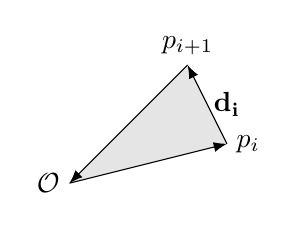
\begin{tikzpicture}

\path [fill=gray!20] (0,0) -- (2,0.5) -- (1.5,1.5) -- cycle;
\draw [-Latex] (0,0) -- (2,0.5);
\node [right] at (2,0.5) {$p_i$};
\draw [Latex-] (0,0) -- (1.5,1.5);
\node [above] at (1.5,1.5) {$p_{i+1}$};
\draw [-Latex] (2, 0.5) -- (1.5,1.5);
\node at (2, 1) {$\bf{d}_i$};
\node [left] at (0,0) {$\mathcal{O}$};

\end{tikzpicture}
\end{document}